\documentclass[a4paper]{article}

% \usepackage{inputenc}
\usepackage[british,UKenglish]{babel}
\usepackage{amsmath}
\usepackage{titlesec}
\usepackage{color}
\usepackage{graphicx}
\usepackage{fancyref}
\usepackage{hyperref}
\usepackage{float}
\usepackage{scrextend}
\usepackage{setspace}
\usepackage{xargs}
\usepackage{multicol}
\usepackage{nameref}

\usepackage{sectsty}
\usepackage{multicol}
\usepackage{multirow}
\usepackage[procnames]{listings}
\usepackage{appendix}
\usepackage{listings}

\newcommand\tab[1][1cm]{\hspace*{#1}}
\hypersetup{colorlinks=true, linkcolor=black}
\interfootnotelinepenalty=10000

\newcommand{\cleancode}[1]{\begin{addmargin}[2em]{2em}\texttt{\textcolor{cleanOrange}{#1}}\end{addmargin}}
\newcommand{\cleanstyle}[1]{\text{\textcolor{cleanOrange}{\texttt{#1}}}}


\usepackage[colorinlistoftodos,prependcaption,textsize=footnotesize]{todonotes}
\newcommandx{\commred}[2][1=]{\textcolor{Red}
{\todo[linecolor=red,backgroundcolor=red!25,bordercolor=red,#1]{#2}}}
\newcommandx{\commblue}[2][1=]{\textcolor{Blue}
{\todo[linecolor=blue,backgroundcolor=blue!25,bordercolor=blue,#1]{#2}}}
\newcommandx{\commgreen}[2][1=]{\textcolor{OliveGreen}{\todo[linecolor=OliveGreen,backgroundcolor=OliveGreen!25,bordercolor=OliveGreen,#1]{#2}}}
\newcommandx{\commpurp}[2][1=]{\textcolor{Plum}{\todo[linecolor=Plum,backgroundcolor=Plum!25,bordercolor=Plum,#1]{#2}}}

\def\code#1{{\tt #1}}

\def\note#1{\noindent{\bf [Note: #1]}}

\makeatletter
%% The "\@seccntformat" command is an auxiliary command
%% (see pp. 26f. of 'The LaTeX Companion,' 2nd. ed.)
\def\@seccntformat#1{\@ifundefined{#1@cntformat}%
   {\csname the#1\endcsname\quad}  % default
   {\csname #1@cntformat\endcsname}% enable individual control
}
\let\oldappendix\appendix %% save current definition of \appendix
\renewcommand\appendix{%
    \oldappendix
    \newcommand{\section@cntformat}{\appendixname~\thesection\quad}
}
\makeatother

\lstdefinelanguage{Julia}%
  {morekeywords={abstract,break,case,catch,const,continue,do,else,elseif,%
      end,export,false,for,function,immutable,import,importall,if,in,%
      macro,module,otherwise,quote,return,switch,true,try,type,typealias,%
      using,while,|>, .|>, =>, ->},%
   sensitive=true,%
   % alsoother={$},%
   morecomment=[l]\#,%
   morecomment=[n]{\#=}{=\#},%
   morestring=[s]{"}{"},%
   morestring=[m]{'}{'},%
}[keywords,comments,strings]%

\lstset{%
    language         = Julia,
    basicstyle       = \fontfamily{Fira Code},
    keywordstyle     = \bfseries\color{blue},
    stringstyle      = \color{magenta},
    commentstyle     = \color{green},
    showstringspaces = false,
}

\lstset{frame=, basicstyle={\footnotesize\ttfamily}}



\graphicspath{ {images/} }
\usepackage{ctex}
\usepackage{fontspec}
% \usepackage[clean]{svg}
\setmonofont[
  Contextuals={Alternate}
]{Fira Code}
%-----------------------------------------BEGIN DOC----------------------------------------

\begin{document}
\renewcommand{\contentsname}{目\ 录}
\renewcommand{\appendixname}{附录}
\renewcommand{\appendixpagename}{附录}
\renewcommand{\refname}{参考文献}
\renewcommand{\figurename}{图}
\renewcommand{\tablename}{表}
\renewcommand{\today}{\number\year 年 \number\month 月 \number\day 日}

\title{{\Huge 数据挖掘实验实验报告{\large\linebreak\\}}{\Large 实验二 Apriori算法\linebreak\linebreak}}
%please write your name, Student #, and Class # in Authors, student ID, and class # respectively
\author{\\姓\ 名:柴\ 博\ 文\\
    学\ 号: 04194012\\
    班\ 号: 大数据1901\\\\
    数据挖掘与机器学习\\
    (秋季, 2021)\\\\
    西安邮电大学\\
    计算机学院\\
    数据科学与大数据专业}
\date{\today}
\maketitle
\newpage

%-----------------------------------------ABSTRACT-------------------------------------
\begin{center}
    {\Large\bf{摘\ 要\\}}
\end{center}

本次实验代码均可以在\href{https://github.com/lovebaihezi/lab/tree/main/data-process/apriori}{github仓库}下找到.

\newpage
%-----------------------------------------CONTENT-------------------------------------
\begin{center}
    \tableofcontents\label{c}
\end{center}
\newpage

%------------------------------------------TEXT--------------------------------------------

%----------------------------------------OVERVIEW-----------------------------------------

\section{概述} \label{overview}%------------------------------

\begin{itemize}
    \item {
          \textbf{算法简述}
          Apriori算法将会从你所给的数据集当中生成频繁项集,频繁项集为由数据集当中原子数据组成的不重复集合,
          并计算这些项集在数据集当中出现的频率(即当前项集的支持度),随后在将这些项集中出现频率大于最小支持度的去掉,
          在将剩下的进行组合,将组合的项集再进行计算,知道在也不能组合生成新的项集.在频繁项集生成之后,再使用频繁项集
          生成关联规则(对于频繁项集X, Y(两者),同时出现(X,Y)的概率,相对与只出现Y的频率).
          }
    \item {
          \textbf{算法流程}
          首先需要从数据集当中生成频繁1项集,计算频繁n项集的支持度,再通过当前频繁n项集计算频繁n项集(合并当前频繁n-1项集,
          不合并多项不同的),然后再遍历所有的频繁项集,求频繁n项集和频繁n-k项集的差集,在算出支持度和提升度
          }
\end{itemize}

\newpage

\section{频繁项集生成} \label{item set generate}

首先是从数据集生成频繁1项集

\begin{lstlisting}[language=julia]
# 合并数据集中的每一项,并进行散列去重
C1::Set{Set{T}} = (∪(data...) .|> v -> Set([v])) |> Set
dict = scan(data, C1, ε) # 生成的频繁1项集的支持度散列表
\end{lstlisting}

对于数据形如

\begin{table}[h]
    \centering
    \begin{tabular}{ |c|c| }
        index & Vector         \\hline
        1     & :A, :C, :D     \\
        2     & :B, :C, :E     \\
        3     & :A, :B, :C, :E \\
        4     & :B, :E         \\
    \end{tabular}
\end{table}

生成的频繁一项集机器支持度(去除了支持度小于0.5的项):图\ref{figure:item1set}.

\begin{figure}[h]
    \centering
    \label{figure:item1set}
    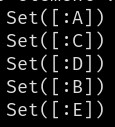
\includegraphics[height=3cm]{item1set.png}
    \caption{频繁1项集的生成}
\end{figure}

接下来,就是根据频繁n-1项集生成频繁n项集

\begin{lstlisting}[language=julia]
for p ∈ L[n-1], q ∈ L[n-1]
    if p != q
        push!(C, p ∪ q) # union sets
    end
end
\end{lstlisting}

然后对频繁n项集进行支持度计算

\begin{figure}[h]
    \centering
    \label{figure:result-itemset}
    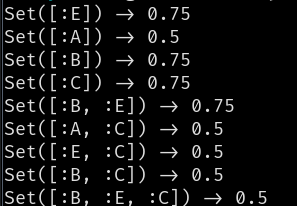
\includegraphics[height=3cm]{result-itemset.png}
    \caption{频繁项集的支持度}
\end{figure}

scan函数参数:
data: 即数据集
C:频繁n项集
$\varepsilon$:最小支持度
scan函数返回值:
返回频繁n项集的KV表, V -> 支持度

\begin{lstlisting}[language=julia]
function scan(
    data::Vector{Vector{T}},
    C::Set{Set{T}},
    ε::Float64,
)::Dict{Set{T},Float64} where {T}
    dict = Dict{Set{T},Float64}()
    data .|> row -> C .|> set -> if set ⊆ row # check each set is subset of each row in data which in C
        v = get!(dict, set, 0) + 1 # Int, yes, set default if is missing, and get value
        dict[set] = v
    end
    len = data |> length # Int, get data set size
    for (key, value) ∈ dict # Vector{T} => Float64, cal each sets support%
        support = value / len
        dict[key] = support
    end
    dict |> keys .|> key -> if dict[key] < ε # remove set which support less than ε
        delete!(dict, key)
    end
    dict
end
\end{lstlisting}

\newpage

\section{关联规则生成} \label {rule generate}

关联规则的生成需要所有频繁$[1-n]$项集的支持度,以及$[1-n]$级频繁项集对应的支持度表

进行便利操作,对于频繁n项集的表中的每一个元素n-set,与所有频繁项集的每一个set分别取差集,

n-set $\Longrightarrow$  set即为一个关联关系

rules函数的入参:
dicts: 频繁n项集与其支持度的表的集合
support:所有频繁项集与其支持度的集合
$\varsigma$:最小置信度

rules函数的返回值
所有关联规则与其支持度和提升度组成的表

\begin{figure}[h]
    \centering
    \label{figure:rules}
    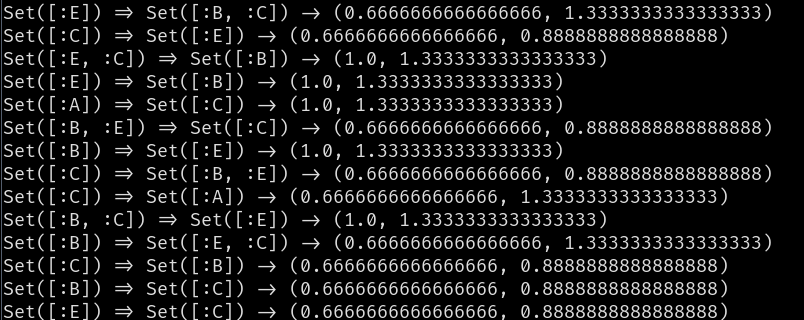
\includegraphics[height=5cm]{rules.png}
    \caption{关联规则结果图(数据同上)}
\end{figure}

\begin{lstlisting}[language=julia]
function rules(
    dicts::Vector{Dict{Set{T},Float64}},
    support::Dict{Set{T}, Float64},
    ς::Float64
   )::Dict{Pair{Set{T},Set{T}}, Tuple{Float64, Float64}} where {T}
    result = Dict{Pair{Set{T}, Set{T}},Tuple{Float64, Float64}}()
    for i ∈ 2:(dicts |> length)
        for x ∈ 1:i-1
            for set ∈ dicts[x] |> keys
                for n_set ∈ dicts[i] |> keys
                    if set ⊆ n_set
                        diff = setdiff(n_set, set)
                        # set ∪ diff = n_set
                        # confidence(set => diff) = count(n_set) / count(set)
                        # (n_set, set => diff, support[n_set] / support[set]) |> println
                        confidence = support[n_set] / support[set]
                        if confidence >= ς
                            result[set => diff] = confidence, confidence / support[diff]
                        end
                    end
                end
            end
        end
    end
    result
end

\end{lstlisting}

\newpage

\section{代码} \label {code}

\begin{lstlisting}[language=julia]
#=
main:
- Julia version: 1.6.3
- Author: lqxc
- Date: 2021-10-19
=#

# D means the whole dataset, which should be Vector{Vector{T}}
# ! count(X) = filter(D, X ⊆ _).count()
# support(X => Y) = count(X ∪ Y) / |D|
# confidence(X => Y) = count(X ∪ Y) / count(X)

function rules(
    dicts::Vector{Dict{Set{T},Float64}},
    support::Dict{Set{T}, Float64},
    ς::Float64
   )::Dict{Pair{Set{T},Set{T}}, Tuple{Float64, Float64}} where {T}
    result = Dict{Pair{Set{T}, Set{T}},Tuple{Float64, Float64}}()
    for i ∈ 2:(dicts |> length)
        for x ∈ 1:i-1
            for set ∈ dicts[x] |> keys
                for n_set ∈ dicts[i] |> keys
                    if set ⊆ n_set
                        diff = setdiff(n_set, set)
                        # set ∪ diff = n_set
                        # confidence(set => diff) = count(n_set) / count(set)
                        # (n_set, set => diff, support[n_set] / support[set]) |> println
                        confidence = support[n_set] / support[set]
                        if confidence >= ς
                            result[set => diff] = confidence, confidence / support[diff]
                        end
                    end
                end
            end
        end
    end
    result
end

#=
# scan the data with each item set in item set set,
# and get each support
=#

function scan(
    data::Vector{Vector{T}},
    C::Set{Set{T}},
    ε::Float64,
)::Dict{Set{T},Float64} where {T}
    dict = Dict{Set{T},Float64}()
    data .|> row -> C .|> set -> if set ⊆ row # check each set is subset of each row in data which in C
        v = get!(dict, set, 0) + 1 # Int, yes, set default if is missing, and get value
        dict[set] = v
    end
    len = data |> length # Int, get data set size
    for (key, value) ∈ dict # Vector{T} => Float64, cal each sets support%
        support = value / len
        dict[key] = support
    end
    dict |> keys .|> key -> if dict[key] < ε # remove set which support less than ε
        delete!(dict, key)
    end
    dict
end

function apriori(
    data::Vector{Vector{T}};
    ε::Float64 = 0.5,
    ς::Float64 = ε,
)::Tuple{
    Vector{Dict{Set{T}, Float64}},
    Dict{Pair{Set{T},Set{T}}, Tuple{Float64, Float64}}
} where {T}
    n = 2
    C1::Set{Set{T}} = (∪(data...) .|> v -> Set([v])) |> Set
    support = Dict{Set{T}, Float64}()
    dict = scan(data, C1, ε)
    merge!(+, support, dict)
    L::Vector{Set{Set{T}}} = [[(dict |> keys)...] |> Set]
    D::Vector{Dict{Set{T},Float64}} = [dict]
    while L[n-1] |> length != 0
        C = Set{Set{T}}()
        # len = L[n-1] |> length
        for p ∈ L[n-1], q ∈ L[n-1]
            if p != q
                push!(C, p ∪ q)
            end
        end
        dict = scan(data, C, ε)
        merge!(+, support, dict)
        push!(D, dict)
        push!(L, [keys(dict)...] |> Set)
        n += 1
    end
    D, rules(D, support, ς)
end

# data = readlines("files/groceries.csv") .|> s -> split(s, ",")

# apriori(data; ε = 0.03, ς = 0.2) .|> 
# [
#    dicts -> dicts .|> dict -> dict |> keys .|> key -> println(key, " -> ", dict[key]),
#     dict -> dict |> keys .|> key -> println(key, " -> ", dict[key])
# ]
apriori([[:A, :C, :D], [:B, :C, :E], [:A, :B, :C, :E], [:B, :E]]; ε = 0.5) .|>
[
    dict -> dict .|> dict -> dict |> keys .|> key -> println(key, " -> ", dict[key]),
    dict -> dict |> keys .|> key -> println(key, " -> ", dict[key])
]

\end{lstlisting}

%------------------------------------Lab Process--------------------------------------

\end{document}

